\documentclass{article}
\usepackage[utf8]{inputenc}
\usepackage[spanish]{babel}
\usepackage{amsmath,amssymb,amsfonts} %Fonts de AMS
\usepackage{mathbbol} %Font para matrices como la identidad
%%Formato de hoja%%
\usepackage[margin=2cm]{geometry}

%%Imagenes%%
\usepackage{graphicx}
\usepackage{wrapfig}
\usepackage{caption}
\usepackage{subcaption}
\graphicspath{{./fig/}}
\usepackage{float}

%%Ecuaciones y teoremas
\numberwithin{equation}{section} %Número de ecuación por sección
\renewcommand{\vec}[1]{\boldsymbol{#1}}
\newcommand{\bb}[1]{\boldsymbol{#1}}


\title{Notas de Incertezas y teoría de errores en Física Experimental}
\author{S. Schiavinato}
\date{}

\begin{document}
\maketitle
\tableofcontents

\section{Probabilidad de eventos}
Sea un conjunto $\Omega$, \emph{conjunto universal}, definimos un $\sigma$-álgebra como un subconjunto cerrado frente a uniones y complementos, es decir:
\begin{equation}
\begin{gathered}
    \forall A \in S \Rightarrow \overline{A} \in S \\
    \forall A_i \in S \Rightarrow \bigcup_{i=0}^{\infty} A_i \in A
\end{gathered}
\end{equation}
y sobre este conjunto definimos una probabilidad como una función a los reales con las siguientes propiedades
\begin{equation}
\begin{gathered}
p(A) \geq 0 \quad \forall A \in S \\
p(A \cup B) = p(A) + p(B) \quad A, B \in S \;/\; A \cap B = \emptyset \\
p(\Omega) = 1
\end{gathered}
\end{equation}

Se puede deducir otras propiedades de esta definición, usando algebra de grupos
\begin{equation}
\begin{gathered}
p(A \cap B) = p(A) + p(B) - p(A \cup B) \\
p(A - B) = p(A) - p(B) \quad p(B)\leq p(A)\\
p(\emptyset) = 0
\end{gathered}
\end{equation}

Definida la probablidad, definimos una \emph{variable aleatoria} $X$ como una relación entre un elemento de la $\sigma$-algebra a los reales, que representa a los elementos del conjunto. La variable aleatoria va a ser nuestra herramienta central, el ladrillo fundador de toda la teoría.

\subsection{Probabilidad condicional, indepedencia}
La probabilidad de un evento $A$ dado que pasó un evento $B$, del mismo espacio muestral, se nota y se calcula como
\begin{equation}
p(A|B) = \frac{p(A \cap B)}{p(B)}
\end{equation}
y se denomina \emph{probabilidad condicional}.

Se define \emph{independencia} de dos eventos $A$ y $B$ como
\begin{equation}
p(A|B) = p(A) \Leftrightarrow p(B|A) = p(B) \Leftrightarrow p(A \cap B) = p(A) p(B)
\end{equation}
siendo todas las expresiones equivalentes. 

Si dos eventos no son independientes, para calcular la probabilidad de $B$ dado $A$ debemos usar el teorema de Bayes
\begin{equation}
p(B|A) = \frac{p(A|B) p(B)}{p(A)}
\end{equation}
Para deducir este teorema solo es necesario escribir la probabilidad condicional en ambos casos.

Una propiedad interesante es que podemos escribir una probabilidad como la suma de probabilidades de otros conjuntos, si estos son \emph{exhautivos}, es decir
\begin{equation}
B_i, B_j \; / \; B_i \cap B_j = \emptyset \qquad \bigcup_{i = 1}^{N} B_i = \Omega
\end{equation}
por lo que podemos escribir la probabilidad de un evento
\begin{equation}
p(A) = \sum_{i = 1}^{N} p(B_i) p(A | B_i)
\end{equation}
\section{Probabilidad de variables continuas}
Para conjuntos infinitos, numerables o densos, podemos definir la probabilidad a partir de la variable aleatoria $X$ como
\begin{equation}
p(X = t= p(\omega / \omega \in \Omega ^ X(\omega) = t)
\end{equation}
Con esta definición tenemos que considerar que no podemos definir la probabilidad de todos los puntos de la recta numérica, salvo un conjunto numerable de puntos. 

En este contexto, definimos la \emph{función acumulativa de probabilidad} como
\begin{equation}
F_X(t) = p(X \leq t)
\end{equation}
por lo que nos permite escribir la probabilidad de un intervalo de la recta numérica como
\begin{equation}
p(a \leq X \leq b) = F_X(b) - F_X(a) + p(x = a)
\end{equation}
donde la probabilidad de $x = a$ queda a libre elección. En la práctica vamos a elegir la probabilidad $p(x=x_i) = 0$.

Con la función acumulativa de probabilidad podemos definir la probabilidad de una variable aleatoria discreta (o conjunto numerable finito o infinito de puntos) con
\begin{equation}
p(X = a) = F_X(a) - F_X(a^{-})
\end{equation}
es decir una discontinuidad en el punto $x = a$

Ahora si definimos la función distribución de probabilidad como
\begin{equation}
f_X(t) = \left.\frac{dF_X}{dx}\right|_t
\end{equation}
que nos permite definir la probabilidad como
\begin{equation}
f_X(x) dx = p(x < X < x + dx) \quad \Rightarrow \quad p(a < X < b) = \int_{a}^{b} f_X(t) dt
\end{equation}
\subsection{Media, mediana y cuantiles}
De una variable aleatoria podemos definir otras nuevas variables, que representan la localización de la probabilidad. La más usada, ya que está expresada en las fórmulas de las distribuciones, es la \emph{esperanza}, \emph{valor esperado} o \emph{valor medio} (por lo tanto en inglés es \emph{mean}), que se define como
\begin{equation}
E(X) = E(x) = \mu = \langle X \rangle = \int_{X} x f_X(x) dx
\end{equation}
que representa intuitivamente el valor más probable que uno puede obtener.

También podemos definir los \emph{$\alpha$-cuantiles} como
\begin{equation}
X_\alpha \equiv p(X < X_\alpha) = \int_{-\infty}^{x_\alpha} f_X(x)dx = \alpha 
\end{equation}
que representan los valores de la variable aleatoria que tienen a su izquierda $\alpha$ probabilidad. La \emph{mediana} es el $0.5$-cuantil, que dividie a la mitad la probabilidad.

La función cuantil la podemos definir como
\begin{equation}
F^{-1}_X(p) = \inf\{x \in \mathbb{R} : p \leq F_X(x)\}
\end{equation}
que generaliza todos los $\alpha$-cuantiles.
\subsection{Varianza, momentos superiores}
Se definen el momento de orden $k$ como
\begin{equation}
\mu'_k = E(X^k) = E(x^k) = \int_{X} x^k f_X(x) dx
\end{equation}
y los \emph{momentos centrados} de orden $k$ como
\begin{equation}
\mu_k = E((X - E(X))^k) = E((x - E(x))^k) = \int_{X} (x - E(X))^k f_X(x) dx
\end{equation}

Con esta definición queda claro que el momento $\mu'_1 = \mu$ es la esperanza, y nombramos \emph{varianza} al momento $\mu_2$, es decir el momento centrado de orden 2
\begin{equation}
Var(X) = \sigma^2 = E((X - E(X))^2) = E(X^2) - E(X)^2 = \int_{X} (x - E(X))^2 f_X(x) dx
\end{equation}
donde se denomina \emph{desviación estándar} a $\sigma$, que es útil porque estima el error de una magntiud a estar en las mismas unidades.

Definida la varianza podemos demostrar que para cualquier variable aleatoria
\begin{equation}
p(|x - \mu|>\epsilon) \leq \frac{\sigma^2}{\epsilon^2}
\end{equation}
resultado qeu se llama teorema de Tchebisheff. Para demostrarlo creamos un intervalo cerrado de medida $2c$ centrado en $\mu$, es decir $[\mu - c, \mu + c]$. La varianza en este caso es, por el teorema del valor medio
\[\sigma^2 = \int_{-\infty}^{\infty} (x - \mu)^2 f_X(x) dx \geq \int_{-\infty}^{\mu - c} (x - \mu)^2 f_X(x) dx + \int_{\mu + c}^{\infty} (x - \mu)^2 f(x) dx\]
Como $x < \mu - c$, entonces $c < |x - \mu|$, por lo tanto $c^2 < |x - \mu|^2 = (x - \mu)^2$. Lo mismo para el otro término, lo que nos queda que 
\[\sigma^2 \geq c^2 \int_{-\infty}^{\mu - c} f_X(x) dx + c^2 \int_{\mu + c}^{\infty} f(x) dx\]
es decir
\[\sigma^2 \geq c^2 (p(x < \mu - c) + p(x > \mu + c)) \]
que finalmente nos queda
\[\sigma^2 \geq c^2 p(|x - \mu | > c)\]
que es lo que buscamos
\section{Probabilidad de varias variables}
Para varias variables aleatorias podemos definir la función acumulativa conjunta como
\begin{equation}
F_{XY}(u,v) = p((x \leq u) \cap (y \leq v)) = p(x \leq u, y \leq v)
\end{equation}
y si definimos la función distribución de probabilidad conjunta como
\begin{equation}
f_{XY}(u,v) = \left.\frac{\partial F_{XY}(x,y)}{\partial x \partial y}\right|_{x = u, y = v}
\end{equation}
con la siguiente propiedad fundamental
\begin{equation}
p(a \leq X \leq b, c \leq Y \leq d) = \int^b_a \int^d_c f_{XY}(x,y) dx dy
\end{equation}
Para más variables es el mismo argumento, con vectores de variables aleatorias $\underline{X}$.
\begin{equation}
p(\underline{a} \leq \underline{X} \leq \underline{b}) = \int_{\underline{a}}^{\underline{b}} f(\underline{x}) d\underline{x}
\end{equation}

Podemos también pasar de varias variables a menos, \emph{marginalizado}, por medio de
\begin{equation}
f_X(x) = \int_{-\infty}^{\infty} f_{XY}(x,y) dy
\end{equation}
y lo mismo para la variable $y$. Para $N$ variables $\underline{X}$, podemos reducirlo a $N-1$ variables con $N-1$ integraciones en el dominio de cada variable.

La definición de esperanza y cuantiles sigue siendo válida para varias variables
\begin{equation}
E(X_i) = E(x_i) = \mu_i = \int t_i f_{\underline{X}}(\underline{t}) d\underline{t}
\end{equation}

También podemos definir la esperanza conjunta como
\begin{equation}
E(X_i X_j) = E(x_i x_j) = \mu_{ij} = \int t_i t_j f_{\underline{X}}(\underline{t}) d\underline{t}
\end{equation}

La probabilidad condicionada podemos definirla con el mismo proceso
\begin{equation}
f_{X|Y} = \frac{f_{XY}}{f_{Y}}
\end{equation}
y por lo tanto la esperanza condicionada
\begin{equation}
E(X|Y) = \int_{-\infty}^{\infty} x f_{X|Y}(x) dx
\end{equation}
La esperanza condicional es una variable aleatoria de $Y$, por lo que podemos encontrar que
\begin{equation}
E(E(x|y)) = E(x)
\end{equation}
a partir de calcular las integrales específicas, para cualquier set de variables aleatorias. Esto se denomina \emph{ley de la expectativa total}.

El teorema de Bayes extendido para varias variables por lo tanto es
\begin{equation}
f_{Y|X}(y, x) = \frac{f_{X|Y}(y, x) f_Y(y)}{f_{X}(x)} = \frac{ f_{X|Y}(x,y) f_Y(y)}{\int f_{X|Y}(x, t) f_Y(t) dt}
\end{equation}

La definición de \emph{independencia} para varias variables la podemos pensar como
\begin{equation}
F_{XY} = F_{X} F_{Y} \qquad f_{XY} = f_X f_Y
\end{equation}
\subsection{Covarianza}
Además de la varianza para cada variable, podemos definir la varianza entre dos variables, denominada \emph{covarianza}
\begin{equation}
\text{Cov}(x_i, x_j) = V_{i,j} = \int \int (x_i - \mu_i) (x_j - \mu_j) f(\underline{x}) d\underline{x} = E(X_i X_j) - E(X_i) E(X_j)
\end{equation}
donde queda claro que
\begin{equation}
\text{Cov}(x_i, x_i) = \text{Var}(x_i) = \sigma^2_i
\end{equation}
La notación $V_{i,j}$ hace alusión a la representación matricial de la covarianza, que corresponde a una matriz real simétrica con elementos de diagonal mayores a cero, lo que nos asegura que sea diagonalizable (y por lo tanto invertible). 

La covarianza puede ser una magnitud positiva, negativa o nula, dependiendo de la dependencia de las variables. Si son independientes es automático que es nula (pero no vale la vuelta). Para conmesurar la dependencia entre variables definimos la \emph{correlación} como
\begin{equation}
\rho = \frac{\text{Cov}(x_i, x_j)}{\sigma_i \sigma_j}
\end{equation}
que puede variar entre -1 y 1. Para ver eso usamos que, deducible a partir de la definición, la varianza de
\begin{equation}
\text{Var}(a x_i + b x_j) = a^2 \text{Var}(x_i) + \text{Var}(x_j) + 2 a b \text{Cov}(x_i, x_j)
\end{equation}
para
\[\text{Var}(k x + y) = k^2 \text{Var}(x) + \text{Var}(y) + 2 k \text{Cov}(x,y) \geq 0 \]
y como es una cuadrátrica mayor a cero para todo valor de $k$, tenemos que
\[ (2 \; \text{Cov}(x,y))^2 - 4 \text{Var}(x) \text{Var}(y) \leq 0 \]
es decir
\[ \frac{(\text{Cov}(x,y))^2}{\text{Var}(x) \text{Var}(y)} \leq 1 \]

Si las variables aleatorias son independientes la correlación es nula, pero una correlación nula no implica independencia de variables. Correlación positiva implica que al aumentar el valor de una variable aumenta el valor de la otra, y correlación negativa implica lo contrario.

\subsection{Cambio de variables}
Si tenemos un set de variables $\underline{X}$, y otras variables $\underline{U}$, para obtener la función distribución de la variables $\underline{U}$ a partir de la de $\underline{X}$ podemos usar la conservación de la probabilidad
\begin{equation}
f_{\underline{X}}(\underline{x}) d\underline{x} = f_{\underline{U}}(\underline{u}) d\underline{u}
\end{equation}
lo que finalmente nos queda
\begin{equation}
f_{\underline{U}}(\underline{u}) = f_{\underline{X}}(\underline{x}(\underline{u})) \left|\frac{d \underline{x}}{d \underline{u}}\right|
\end{equation}
donde la derivada es el jacobiano de la transformación inversa. Esto es un caso particular del teorema de la función inversa.
\section{Propagación de errores}
Si tengo un set nuevo de variables aleatorias $\underline{y}$ relacionado con las variables aleatorias originales por
\begin{equation}
\underline{y} = F(\underline{x})
\end{equation}
podemos expresar cada componente de $\underline{y}$, por el teorema de Taylor, como 
\[y_l = y_l(\underline{x}) = y_l(\underline{\mu}) + \sum_{i = 1}^{N} \left.\frac{\partial y_l}{\partial x_j}\right|_{\underline{\mu}} (x_i - \mu_i) + O((x_i - \mu_i)^2)\]
por lo tanto
\[y_l - y_l(\underline{\mu}) = \sum_{i = 1}^{N} \left.\frac{\partial y_l}{\partial x_j}\right|_{\underline{\mu}} (x_i - \mu_i) + O((x_i - \mu_i)^2)\]
Multiplicamos $y_l$ y $y_k$ de esta forma y tomamos valores medios, que implica integrar a ambos lados, deducimos que

\begin{equation}
\text{Cov}(y_l,y_k) = \sum_{i,j}  \left.\frac{\partial y_l}{\partial x_i}\right|_{\underline{\mu}}  \left.\frac{\partial y_k}{\partial x_j}\right|_{\underline{\mu}}  \text{Cov}(x_i,x_j)
\end{equation}

\section{Teorema central del límite}
\subsection{Función característica. Función generadora de momentos}
Podemos definir una nueva función asociada a la función distribución de probabilidades, denominada función característica como
\begin{equation}
\phi_{X}(t) = E(e^{i t x}) = \int_{-\infty}^{\infty} e^{i t x} f_{X}(x) dx
\end{equation}
que es trivial extender a varias dimensiones (al menos la notación)
\begin{equation}
\phi_{\underline{X}}(\underline{t}) = E(e^{i t \underline{X}}) = \int_{\text{Dom}\{\underline{X}\}} e^{i t \underline{x}} f_{\underline{X}}(\underline{x}) d x
\end{equation}

Esta función característica representa una tranformada de Fourier de la distribución de probabilidades, por lo que la antitransformada nos da
\begin{equation}
f_{X}(x) = \frac{1}{2\pi} \int_{\infty}^{\infty} e^{-i t x} \phi_{X}(t) dt
\end{equation}

La función característica nos permite encontrar los momentos de una variable aleatoria (usando que la esperanza es lineal, como es natural de su definición) de forma fácil
\[\frac{d \phi_{X}(t)}{dt} = E\left( \frac{d}{dt} e^{i t x}\right) = E(i x e^{i t x}) = i E(x e^{i t x}) \]
por lo que podemos concluir que
\begin{equation}
E(x^k) = i^k \left.\frac{d^{k} \phi_{X}(t)}{dt^{k}}\right|_{t=0}
\end{equation}

Otra propiedad importante es la función característica de una función lineal de variables aleatorias independientes. Sea \[Z = a X + b Y,\] con $a, b$ numeros reales constantes. La función característica de $Z$ será \[ \phi_{Z}(t) = E(e^{i t Z}) = E(e^{i t (a X + b Y)}) = E(e^{i t a X} e^{i t b Y}) = E(e^{i t a X}) E(e^{i t b Y}) = \phi_{X}(a t) \phi_{Y}(b t)\]
Es decir
\begin{equation}
S = \sum_{i} a_i X_i \; \Rightarrow \; \phi_{S}(t) = \prod_{i} \phi_{X_i}(a_i t)
\end{equation}.

La función generadora de momentos de una variable discreta la definimos como
\begin{equation}
G_{X}(t) = E(t^x) = \sum_{x = 1}^{\infty} t^x p(x) 
\end{equation}
que se relaciona con la función característica con
\begin{equation}
\phi_{X}(t) = G_{X}(z = e^{i t})
\end{equation}
por lo que los momentos son
\begin{equation}
\mu_k = \left.\frac{d^{k} G_{X}}{dz^k}\right|_{z=1}
\end{equation}
Una función lineal de variables aleatorias discretas siguen verificando que
\begin{equation}
S = \sum_{i} a_i X_i \; \Rightarrow \; G_{S}(z) = \prod_{i} G_{X_i}(z^{a_i})
\end{equation}
pero además si tengo que la cantidad de variables aleatorias, que ahora las consideramos independientes e \emph{identicamente} distribuidas (i.i.d), es aleatoria, que representamos con $N$, podemos deducir, usando la esperanza condicional
\begin{equation}
S = \sum^N_{i=1} X_i \; \Rightarrow \; G_{S}(t) = G_N(G_{X}(z))
\end{equation}
\subsection{Teorema central del límite}
Dada una variable $X$, la función característica la podemos expresar como una serie de potencias respecto a $t = 0$ como
\[\phi_{X}(t) = \phi_{X}(0) + \left.\frac{d \phi_{X}(t)}{d t}\right|_{t=0} t + \left.\frac{d^2 \phi_{X}(t)}{d t^2}\right|_{t=0} t^2 + O(t^3) = 1 + \mu_1 t + \mu_2 t^2 + O(t^3) \]
Podemos hacer lo mismo para el logaritmo del la función característica
\[\log(\phi_X(t)) = \log(\phi_X(0)) + \left.\frac{d \log(\phi_X(t))}{dt}\right|_{t=0} t + \left.\frac{d^2 \log(\phi_X(t))}{dt^2}\right|_{t=0} t^2 + O(t^3)\]
Si usamos la regla de la cadena nos va quedando 
\begin{equation}
\log(\phi_X(t)) = i \mu t - \frac{\sigma}{2} t^2 - \frac{i}{6} M_3 t^3 + \frac{1}{24} M_4 t^4 + \dots = \sum_{k=0}^{\infty} \frac{t^k}{k!} i^k M_k
\end{equation}
siendo $M_k$ los \emph{momentos cumulantes} que para los primeros tres son igual a los momentos centrados.

De importancia capital es saber que la distribución normal o gaussiana
\begin{equation}
f(x) = N(x|\mu, \sigma) = \frac{1}{\sqrt{2 \pi} \sigma} \exp\left(\frac{1}{2}\left(\frac{x - \mu}{\sigma}\right)^2\right)
\end{equation}
tiene la siguiente función característica
\begin{equation}
\phi(t) = \exp\left(i \mu t - \frac{\sigma^2}{2} t^2\right)
\end{equation}
por lo que la suma de normales es una normal, es decir
\begin{equation}
X_i \sim N(\mu_i, \sigma_i) \; \Rightarrow \; \sum_i X_i \sim N\left(\mu = \sum_i \mu_i\,,\; \sigma = \sqrt{\sum_i \sigma^2_i}\right)
\end{equation}

Ahora si tengo una variable $Z$ con varianza $\sigma^2$ y esperanza $\mu$ definida, puedo transformarla en una variable $Y$ con varianza $1$ y esperanza $0$ por medio de
\begin{equation}
Y = \frac{Z - \mu}{\sigma}
\end{equation}
que es fácil de deducir a partir de la fórmula general de cambio de variables y la definición de varianza y esperanza.


Con estas herramientas, para probar el \emph{teorema central del límite}, que corresponde a que la suma de variables con momentos acotados tiende a ser una variable normal, tenemos un conjunto de variables $X_i$ i.i.d, con $E(x) = \mu$ y $\text{Var}(x) = \sigma$ (es un caso especial, que puede ser extendido al caso general)

Construimos la suma de todas las variables \[Z = \sum_{i} X_i \]
y a continuación hacemos el siguiente cambio de variables 
\[Y = \frac{Z - E(Z)}{\sqrt{\text{Var}(Z)}} \]
por lo tanto 
\[ \phi_{Y} = E\left(e^{i t \frac{\sum_{i} X_i - \mu}{\sqrt{n} \sigma}}\right) = \prod_i \phi_{X_i - \mu}\left(\frac{t}{\sqrt{n} \sigma}\right)\]
por lo que el logaritmo será
\[\log(\phi_{Y}) = \sum_i \log\left(\phi_{X_i - \mu}\left(\frac{t}{\sqrt{n} \sigma}\right) \right) = \sum^{n}_{i=1} \left[ -\frac{1}{2} \frac{t^2}{n \sigma^2} \sigma^2 + O\left(\frac{t^3}{n^{3/2} \sigma}\right) \right] = -\frac{1}{2} t^2 + O\left(\frac{t^3}{n^{3/2 - 1} \sigma}\right) \xrightarrow[n\to\infty]{}  -\frac{1}{2} t^2\]
es decir que la distribución de $Y$ es una normal $N(0,1)$, por lo que la distribución de $Z$ tiende a una normal $N(\mu = \sum_i \mu_i, \sigma = \sqrt{\sum_i \sigma^2_i})$.

Este teorema, que es válido para variables con momentos finitos, se puede extender a muchas variables, no identicamente distribuidas, pero la demostración general exige herramientas matemáticas más avanzadas.


\section{Distribuciones de probabilidades especiales}
\subsection{Distribuciones discretas}

La primer distribución de probabilidad que vamos a conocer se denomina \emph{binomial}, que corresponde a $N$ eventos con probabilidad $p$, constante, de tener un resultado y probabilidad $1 - p$ de obtener otro, independientes entre si los experimentos. Como son todos los eventos son independientes, obtener $k$ éxitos de probabilidad $p$ (como son dos eventos, uno es éxito y otro es fracaso) de $N$ experimentos es igual a
\[ p(k) = p^{k} (1-p)^{N-k}\]
pero eso es la probabilidad de una combinación de éxitos, donde importa el orden de como salieron. Como no nos interesa el orden debemos considerar las combinaciones de ellos
\begin{equation}
p(k) = B(k ; N, p) = \binom{N}{k} p^{k} (1 - p)^{N - k}
\end{equation}
que obviamente está normalizada, ya que
\begin{equation}
\sum_{k = 0}^{N} B(k | N, p) = \sum_{k = 0}^{N} \binom{N}{k} p^k (1 - p)^{N - k} = (p + 1 - p)^{N} = 1
\end{equation}

La esperanza de la distribución binomial corresponde a 
\[ E(k) = \sum_{k = 0}^{N} k B(k | N, p) = \sum_{k = 0}^{N} k \binom{N}{k} p^k (1 - p)^{N - k} \]
para calcularlo consideremos $q = 1- p$, por lo que
\[(p + q)^{N} = \sum_{k = 0}^{N} \binom{N}{k} p^k q^{N - k}\]
ahora derivo respecto a $p$ a ambos lados
\[ N  (p + q)^{N-1} = \sum_{k = 0}^{N} \binom{N}{k} k p^{k - 1} q^{N - k} \]
y multiplicamos por $p$ a ambos lados finalmente
\[ p N (p + q)^{N - 1} = \sum_{k = 0}^{N} p k \binom{N}{k} p^{k - 1} q^{N - k} = \sum_{k = 0}^{N} k \binom{N}{k} p^{k} q^{N - k} = E(k)\]
por lo tanto
\begin{equation}
E(k| k \sim B(N, p)) = N p
\end{equation}
Para calcular la varianza hacemos exactamente el mismo proceso para el valor medio de $k^2$, pero derivando dos veces, y obtenemos
\begin{equation}
\text{Var}(k|k\sim B(N,p)) = N p ( 1 - p)
\end{equation}

Podemos encontrar, de forma directa al aplicar la definición, que la función característica de la binomial corresponde a
\begin{equation}
\phi_{X}(t) = (1 - p + p e^{it})^{N}
\end{equation}

Si tenemos una distribución binomial donde la cantidad de experimentos tiende a infinito, pero la probabilidad de cada evento tiende a cero, encontramos una distribución de Poisson (es más, estos eventos se enmarcan en la \emph{ley de los eventos raros}). Es decir
\begin{equation}
B(N, p) \xrightarrow[D]{N \to \infty, p \to 0 \; / \; N p \to \lambda} P(\lambda)
\end{equation}
donde la $D$ corresponde a límite en distribución, como ya vimos. Para encontrar la distribución de Poisson, sabemos que el coeficiente binomial
\begin{equation}
\lim_{N\to\infty} \binom{N}{k} = \lim_{N\to\infty} \frac{1}{k!} \frac{N!}{(N - k)!} = \lim_{N\to\infty} \frac{1}{k!} \frac{N (N - 1) \cdots (N - k + 1) (N - k) (N - k - 1) \cdots}{(N - k) (N - k - 1) \cdots } = \frac{N^k}{k!}
\end{equation}
y que si la probabilidad tiende a cero
\begin{equation}
\lim_{N\to\infty\;p \to 0} (1 - p)^{N} = \lim_{N\to\infty, p \to 0} (1 - p)^{\frac{\lambda}{p}} = \lim_{N\to\infty, p \to 0} \left[(1 - p)^{\lambda}\right]^{p} = e^{-\lambda}
\end{equation}
donde usamos L'Hopital para resolver el último límite.

Si juntamos todos estos resultados tenemos que
\begin{equation}
P(k;\lambda) = \frac{\mu^{k}}{k!} e^{\mu}
\end{equation}

Si usamos el mismo límite para la esperanza y la varianza de la binomial, llegamos a que
\begin{equation}
\begin{gathered}
E(k|k \sim P(\lambda)) = \lambda \\
\text{Var}(k|k\sim P(\lambda)) = \lambda
\end{gathered}
\end{equation}

Podemos llegar al mismo resultado con funciones características, ya que si tomamos el límite
\begin{equation}
\lim_{N\to\infty\;p\to 0} (1 - p + p e^{it})^N = \lim_{N\to\infty\;p\to 0} (1 + p ( e^{it} - 1))^N = \lim_{N\to\infty\;p\to 0} \left(1 + \frac{N p}{N} (e^{it} - 1 )\right)^N = e^{\lambda (e^{it} - 1)}
\end{equation} 
que podemos encontrar, con un poco de álgebra, que es la función característica de la distribución de Poisson.

\subsection{Distribuciones continuas}
\subsubsection{Normal, multinormal}
La distribución continua más recurrente es la distribución normal, que ya definimos como
\begin{equation}
N(x;\mu,\sigma) = \frac{1}{\sqrt{2 \pi \sigma^2}} \exp\left[\frac{1}{2} \frac{(x - \mu)^2}{\sigma^2}\right]
\end{equation}
donde sabemos que
\begin{equation}
\begin{gathered}
E(x) = \mu \\
\text{Var}(x) = \sigma^2
\end{gathered}
\end{equation}
y además no tiene más momentos, que queda plasmado en la función característica
\begin{equation}
\phi_{X}(t) = e^{i t \mu - \frac{t^2}{2} \sigma^2}
\end{equation}

Esta función generaliza a varias variables, con matriz de covarianza $V$ y vector de esperanzas $\overline{\mu}$ como
\begin{equation}
\mathcal{N}(\overline{x}|\overline{\mu}, V) = \frac{1}{\sqrt{(2\pi)^{k}|V|}}
\exp\left[-\frac{1}{2}(\overline{x}-\overline{\mu})^\mathrm{T} V^{-1} (\overline{x}-\overline{\mu})\right]
\end{equation}
De esta expresión obtenemos la normal en una sola dimensión, pero además podemos ver que todas las variables son normales al serl marginalizadas y además todas las probabilidades conjuntas son normales. La función característica de la multinormal corresponde a
\begin{equation}
\phi_{\underline{X}}(\underline{t}) = \exp\left[i \underline{\mu}^{T} \underline{t} - \frac{1}{2} \underline{t}^T V \underline{t}\right]
\end{equation}

Con las expresiones de función característica de la normal y la multinormal queda claro que la suma (y resta) de variables aleatorias normales es también una variable normal. Además, se puede demostrar que cualquier transformación afín, es decir una transformación lineal más una translación, genera una nueva varialbe
\begin{equation}
\underline{Y} = \underline{c} + B \underline{X}
\end{equation}
que es también multinormal, tal que
\begin{equation}
\underline{Y} \sim \mathcal{N}(\underline{c} + B \underline{\mu}, B V B^{T})
\end{equation}
Con esto último queda definida los cambios de variables lineales de variables normales.

\subsubsection{$\chi^2$, Cauchy, t-student}
En caso de tener una variable aleatoria normal estándar elevada al cuadrado, es decir
\[ X \sim N(0,1) \; \rightarrow \; Z = X^2 \]
Si usamos la fórmula de cambio de variables (considerando que la transformación no es inversible, pero si restringimos a los valores positivos y multiplicamos por dos obtenemos, por simetría, el resultado) tenemos que
\[f_Z(z) = 2 f_X(\sqrt{z}) \left|\frac{d \sqrt{z}}{d z}\right| = \frac{1}{\sqrt{2\pi}\sqrt{z}} e^{-\frac{z}{2}}\]
Podemos hacer el mismo ejercicio para $N$ variables, integrando en esféricas (ya que $Z = r^2$) de $N$ dimensiones, obteniendo
\[f_Z(z) = z^{N/2 - 1} e^{-Z/2} \]
y si normalizamos (integrando en esféricas)
\begin{equation}
\chi^2_{N}(z) = \frac{1}{2^{N/2} \Gamma(N/2)} z^{N/2 - 1} e^{-z/2}
\end{equation}
que corresponde a la distribución $\chi^2$ de $N$ grados de libertad.

Esta distribución es especialmente útil ya que representa la suma al cuadrado de variables aleatorias normales estandar, situación que aparece en el exponente de la función multinormal, por lo que aparece en cuadrados minimos. Además el test $\chi^2$ lleva ese nombre porque el estadístico tiene una distribución $\chi^2$, al ser suma de variables normales estándar al cuadrado. 

La función característica de la $\chi^2$ es particularmente simple
\begin{equation}
\phi_{X}(t) = (1 - 2 i t)^{N/2}
\end{equation}

Ahora, el cociente de variables aleatorias normales estándares, es decir
\begin{equation}
X, Y \sim N(0, 1) \; Z = \frac{X}{Y}
\end{equation}
lo podemos encontrar usando la siguiente regla de transformación
\begin{equation}
f_{X/Y}(z) = \int^{+\infty}_{-\infty} |y|\, f_{X}(zy) f_Y(y) \, dy
\end{equation}
por lo que finalmente nos queda
\begin{equation}
f_Z(z) = \frac{1}{\pi (1 + x^2)}
\end{equation}
distribución que se llama de Cauchy estándar. Esta distribución no tiene ningún momento definido. La distribución general de Cauchy se define
\begin{equation}
f(x; x_0,\gamma) = \frac{1}{\pi\gamma \left[1 + \left(\frac{x - x_0}{\gamma}\right)^2\right]} = { 1 \over \pi \gamma } \left[ { \gamma^2 \over (x - x_0)^2 + \gamma^2  } \right]
\end{equation}
donde $x_0$ es la ubicación del máximo y $\gamma$ es el ancho medio. La función característica de la forma general de Cauchy es
\begin{equation}
\phi_{X}(t) = \exp(x_0\,i\,t-\gamma\,|t|)
\end{equation}

Habiendo definido la distribución $\chi^2$, podemos definir una distribución nueva, igual 
\begin{equation}
T = \frac{X}{\sqrt{V/\nu}}
\end{equation}
siendo $X \sim N(0,1)$ y $V \sim \chi^2_{\nu}$. La distribución de $T$ corresponde a la t-student estándar de grado $\nu$, que tiene la siguiente distribución
\begin{equation}
t(x;\nu) = \frac{\Gamma((\nu+1)/2)}{\sqrt{\nu\pi\,}\,\Gamma(\nu/2)} (1+x^2/\nu)^{-(\nu+1)/2}
\end{equation}

Esta función aparece frecuentemente en la teoría de estimación, por lo que es relevante comentarla.
\subsubsection{Uniforme}
La distribución uniforme corresponde a 
\begin{equation}
X \sim U(a, b) \; \Rightarrow \; f_X(x) = \begin{cases} \frac{1}{b - a} & a < x < b \\ 0 & x > b, x < a \end{cases}
\end{equation}
es decir una distribución que asigna a todos los puntos de un intervalo con la misma probabilidad. La esperanza y varianza de esta distribución corresponde a 
\begin{equation}
\begin{gathered}
E(X|X\sim U(a,b)) = \frac{a + b}{2}\\
\text{Var}(X|X\sim U(a,b)) = \frac{(b - a)^2}{12}
\end{gathered}
\end{equation}
La función característica de esta distribución es
\begin{equation}
\phi_X(t) = \frac{e^{itb}-e^{ita}}{it(b-a)}
\end{equation}
\section{Estimación puntual de estimadores}
En estadística en general tenemos un conjunto de datos, que concentramos en notación con el vector $\underline{x}$, y tenemos parámetros que usualmente queremos determinar, que notamos como $\underline{\theta}$ (también vectorial). Si los conjuntos de datos provienen todos de una distribución y son independientes, podemos definir a la probabilidad conjunta como
\begin{equation}
L(\underline{x}|\underline{\theta}) = \prod_{i = 1}^N f(\underline{x}|\underline{\theta})
\end{equation}
donde en estadística se usa el símbolo $L$ y se la denomina \emph{verosimilitud} (o \emph{likelihood}). Este caso, aunque parezca muy restrictivo, es el problema central de la estadística, además de ser fundamental en todos los teoremas de la inferencia estadística. La notación de $L(\underline{x}|\theta)$ parece que considera al parámetro $\theta$ como una variable aleatoria, pero no es el caso en la interpretación frecuentista (que es la que utilizamos hasta este momento); sin embargo, la notación también nos permite entender a la función verosimilitud como una función del parámetro dados los datos y representa, naturalmente, la probabilidad de dados los datos que el parámetro valga $\theta$.

Ahora, tenemos que una función de los datos $\hat{t}(\underline{x})$, es decir que puede ser \emph{observable} o medible, la llamamos \emph{estadístico} o \emph{estimador}, que nos permite obtener información de estos datos. La notación para estadísticos es diferente debido a que vamos a usar propiedades de ellos considerándolos variables aleatorias, como son en el rigor de la definición. 

En particular, buscamos estimadores que tenga la siguiente propiedad
\begin{equation}
E(\hat{t}(\underline{x})) = f(\underline{\theta})
\end{equation}
es decir que el valor esperando del estimador sea una función de los parámetros.

Vamos a definir algunas propiedades de los estimadores, que nos permite definir una escala de mejor estimadores y poder tomar decisiones.

\subsection{Consistencia}
Dado una sucesión de estimadores, donde vamos cambiando la cantidad de datos, decimos que es consistente si verifica que
\begin{equation}
\forall \epsilon > 0 \; \; \lim_{n\to\infty} P(|\hat{t} - E(\hat{t}| \geq \epsilon) = 0
\end{equation}
es decir que al aumentar a infinito la cantidad de datos la probabilidad el valor del estimador se acerca todo lo que uno quiera al valor esperado. Este límite también se nota
\begin{equation}
X_n \xrightarrow{P} g
\end{equation}

En este sentido sabemos que por la ley de los grandes números que para el estadístico
\begin{equation}
\overline{X} = \frac{1}{n} \sum_{i=1}^{N} x_i
\end{equation}
que se denomina la \emph{esperanza muestral}, y la ley de los grandes números dictamina
\begin{equation}
\lim_{n\to\infty}P(|\overline{x} - \mu|\geq\epsilon) = 0
\end{equation}
es decir que el estimador es consistente. Para ver es podemos calcular la varianza del estimador $\overline{x}$, con
\[\text{Var}(\overline{x}) = \text{Var}\left(\frac{\sum_{i} x_i}{n}\right) = \frac{1}{n^2} \sum_i \text{Var}(x_i) = \frac{n \sigma^2}{n^2} = \frac{\sigma^2}{n}\]
Por la desigualdad de Tschebischeff tenemos que
\[P(|\overline{x} - \mu|\geq \epsilon) \leq \frac{\text{Var}(\overline{x})}{\epsilon^2} = \frac{\sigma^2}{n \epsilon^2} \xrightarrow{n\to\infty} 0\]


\subsection{Sesgo}
Definimos el \emph{sesgo} o \emph{bias} como la diferencia entre la esperanza del estimador y lo estimado, es decir
\begin{equation}
b = E(\hat{t}) - \theta
\end{equation}
En general el sesgo puede ser una función de los parámetros, y además de la cantidad de datos. 

El caso más paradigmático de un estimador sesgado es la varianza muestral sin correción, es decir
\begin{equation}
S^2 = \frac{1}{n} \sum_{i=1}^{N} (x_i - \overline{x})
\end{equation}
Para calcularle la esperanza, partimos de (en notación de indices)
\[(x_i - \overline{x}) = (x_i - \mu + \mu - \overline{x}) = ((x_i - \mu) - (\overline{x} - \mu)) = ((x_i - \mu) - \frac{1}{n} (x_j - \mu))\]
y tomo el cuadrado de esto último
\[(x_i - \mu)^2 + \frac{1}{n^2} (x_j - \mu) (x_k - \mu_) - \frac{2}{n} (x_i - \mu) (x_j - \mu) \]
Tomamos la esperanza, que conmuta con las sumas por ser un operador lineal
\[E((x_i - \mu)^2) + \frac{1}{n^2} E((x_j - \mu)(x_k - \mu)) - \frac{1}{n} E((x_i - \mu)(x_j - \mu))\]
La suma explicita inicial es sobre el índice $i$, por lo que el segundo término contiene solo una componente de la matriz de covarianza, que es diagonal y todos los elementos iguales a $\sigma^2$. El segundo término mientras tanto corresponde a sumar $n$ elementos $\sigma^2$, lo que nos queda
\[E(x_i - \overline{x}) = \sigma^2 + \frac{1}{n^2} n \sigma^2 - \frac{2}{n} \sigma^2\]
que finalmente nos permite deducir que la esperanza del estimador $S^2$ es
\begin{equation}
E(S^2) = \frac{n - 1}{n} \sigma^2
\end{equation}
es decir es un estimador sesgado. Esto se corrige definiendo el estimador, que conocemos como \emph{varianza muestral}
\begin{equation}
s^2 = \frac{1}{n - 1} \sum_{i=1}^{n} x_i - \overline{x}
\end{equation}
que es la versión no sesgada del estimador más "natural" para la varianza.

\subsection{Eficiencia}
Dado un estimador $\hat{t} = \hat{t}(\underline{x})$, queremos calcularle su varianza, para lo que tenemos ante todo su esperanza
\begin{equation}
E(\hat{t}) = h(\theta) + b(\theta) = \int \hat{t}(\underline{x}) L(\underline{x} | \theta) d\underline{x}
\end{equation}
Como es una estadística, consideramos que este quiere estimar una función del parámetro $h(\theta)$, con un sesgo $b(\theta)$. 

Para encontrar el mejor estimador, primero vamos a encontrar el estimador sin sesgo con mínima varianza (MVUE, minimun variance unbiased estimator). Primero vamos a exigir la siguiente regularidad
\begin{equation}
\frac{\partial}{\partial \theta} \int f(\underline{x}) L(\underline{x}|\theta) d\underline =  \int f(\underline{x}) \frac{\partial}{\partial \theta} L(\underline{x}|\theta) d\underline{x}
\end{equation}
que se consigue si los límites de integración no depende del parámetro (como para la mayoría de las distribuciones o verosimilitudes, salvo la distribución uniforme).

Tenemos que
\[ \int L(\underline{x}|\theta) d\underline{x} = 1\]
si derivamos a ambos lados, usando la regularidad
\[ \int \frac{\partial}{\partial \theta} L(\underline{x}|\theta) d\underline{x} = 0\]
Ahora sabemos que por regla de la cadena
\[ \frac{\partial}{\partial \theta} \log L(\underline{x}|\theta) = \frac{1}{L} \frac{\partial}{\partial \theta} L(\underline{x}|\theta)\]
por lo que
\[ \int  L \frac{\partial}{\partial \theta} \log L(\underline{x}|\theta) d\underline{x} = 0\]
Usando nuevamente la regularidad, pero ahora con $E(t) = h(\theta) + b(\theta)$, agregamos
\[ \int (h(\theta + b(\theta) L \frac{\partial}{\partial \theta} \log L(\underline{x}|\theta) d\underline{x} = 0 \]
mientras tenemos que
\[\frac{\partial}{\partial \theta} E(\hat{t}) =  \frac{\partial}{\partial \theta}h(\theta) + \frac{\partial}{\partial \theta} b(\theta) = \frac{\partial}{\partial \theta} \int \hat{t}(\underline{x}) L(\underline{x} | \theta) d\underline{x} = \int \hat{t}(\underline{x}) \frac{\partial}{\partial \theta} L(\underline{x} | \theta) d\underline{x} = \int \hat{t}(\underline{x}) L(\underline{x}|\theta) \frac{\partial}{\partial \theta} \log L(\underline{x} | \theta) d\underline{x}\]

Si restamos esta última expresión con la anterior obtenemos
\[\int [\hat{t}(\underline{x}) - h(\theta) - b(\theta)] L(\underline{x}|\theta) \frac{\partial}{\partial \theta} \log L(\underline{x} | \theta) d\underline{x} = \frac{\partial}{\partial \theta} h + \frac{\partial}{\partial \theta} b\]

Sabemos que dada $f$ y $g$ funciones, la desigualdad de Cauchy Schwarz del producto interno corresponde a 
\begin{equation}
\int |f|^2 dx \int |g|^2 dx \geq \left|\int f g dx \right|^2
\end{equation}
por lo que
\[ \left[ \frac{\partial}{\partial \theta} h + \frac{\partial}{\partial \theta} b \right]^2 =  \left[ \int [\hat{t}(\underline{x}) - h(\theta) - b(\theta)] L(\underline{x}|\theta) \frac{\partial}{\partial \theta} \log L(\underline{x} | \theta) d\underline{x} \right]^2\] \[\leq   \int [\hat{t}(\underline{x}) - h(\theta) - b(\theta)]^2 L(\underline{x}|\theta) d\underline{x} \int \left[\frac{\partial}{\partial \theta} \log L(\underline{x} | \theta)\right]^2 L(\underline{x}|\theta) d\underline{x}\]
De esta última desigualdad, concluimos
\begin{equation}
\text{Var}(\hat{t}) \geq \frac{\frac{\partial}{\partial \theta} h + \frac{\partial}{\partial \theta} b}{E\left( \left[\frac{\partial}{\partial \theta} \log L \right]^2\right)}
\end{equation}
para \emph{cualquier} estimador $\hat{t}$, solo asumiendo que la distribución de los datos verifica la regularidad.
Es decir, dada una distribución de datos con un parámetro $\theta$ y con la condición de la regularidad, todo estimador de una función $h(\theta)$ con un bias $b(\theta)$ tiene a lo sumo una varianza con cota menor a la especificada. Este resultado se llama \emph{cota de Cramer-Rao}. 

Esto nos permite definir la eficiencia, como
\begin{equation}
\epsilon = \frac{\min(\text{Var})}{\text{Var}(\hat{t})}
\end{equation}

La igualdad se obtiene si en la desigualdad de Cauchy-Schwarz se verifica la igualdad, que pasa si ambas funciones son proporcionales. Es decir
\begin{equation}
\frac{\partial}{\partial \theta} \log L(\underline{x}|\theta) = A(\theta) (\hat{t}(\underline{x}) - E(\hat{t}))
\end{equation}

Para varias dimensiones podemos extender la cota de Cramer-Rao con la siguiente expresión
\begin{equation}
\text{Cov}(\underline{\theta}) \geq \frac{\partial E(\hat{t})}{\partial \underline{\theta}} \frac{1}{I[\underline{\theta}]} \frac{\partial E(\hat{t})}{\partial \underline{\theta}}^T
\end{equation}
donde la esperanza del estimador también es un vector aleatorio, por lo que la derivada corresponde a la matriz jacobiana. La matriz $I[\underline{\theta}]$ se denomina \emph{información de Fisher}, que tiene la siguiente expresión general
\begin{equation}
I_{m, k} = E\left[
 \frac{\partial }{\partial \theta_m} \log L\left(\underline{x}|\underline{\theta}\right)
 \frac{\partial }{\partial \theta_k} \log f\left(\underline{x}| \underline{\theta}\right)
\right]
\end{equation}
que para una dimensión (que se extiende a varias) podemos encontrar otra expresión equivalente
\[\frac{\partial}{\partial \theta} \left( L(\underline{x}|\theta) \frac{\partial}{\partial \theta}(\log L(\underline{x}|\theta)) \right) = \frac{\partial}{\partial \theta} L(\underline{x}|\theta) \frac{\partial }{\partial \theta} \log(L(\underline{x}|\theta)) + \frac{\partial^2}{\partial \theta^2}(\log(L(\underline{x}|\theta)) L(\underline{x}|\theta)\]
Si integramos a ambos lados tenemos
\[\int \frac{\partial}{\partial \theta} \left( L(\underline{x}|\theta) \frac{\partial}{\partial \theta}(\log L(\underline{x}|\theta)) \right) d\underline{x} = \int \frac{\partial^2}{\partial \theta^2} L(\underline{x}|\theta)  d\underline{x} = 0\]
\[= \int \left(\frac{\partial}{\partial \theta} L(\underline{x}|\theta)\right)^2 L(\underline{x}|\theta) d\underline{x} \; + \; \int \frac{\partial^2}{\partial \theta^2}(\log(L(\underline{x}|\theta))  L(\underline{x}|\theta) d\underline{x}\]
es decir
\begin{equation}
E\left(\left(\frac{\partial}{\partial \theta} \log L(\underline{x}|\theta)\right)^2\right) = - E\left(\frac{\partial^2}{\partial \theta^2}(\log(L(\underline{x}|\theta))\right)
\end{equation}
es decir que la información de Fisher puede ser también, bajo la condición de regularidad
\begin{equation}
I(\underline{\theta}) = - E\left[ \frac{\partial^2}{\partial\theta_i \, \partial\theta_j} \log L(\underline{x}|\underline{\theta})\right]
\end{equation}
\subsection{Suficiencia}
Puede ser el caso que dado todo los datos $\underline{x}$ no necesitemos todos ellos, es decir toda la información que proveen, para calcular un estimador $\hat{t}$ de alguna función de los parámetros. Un estadístico que sea \emph{suficiente} conservará toda la información de $\underline{x}$ para la estimación de la función.

Formalmente se dice que un estimador es suficiente si la distribución, léase la verosimilitud, de $\underline{x}$ condicionada a que $\hat{t} = t$ (que tenga un valor definido el estimador) es independiente de la función del parámetro que estima la estadística. 

También definimos a un estimador $\hat{t}$ como \emph{suficiente mínimo} si verifica que
\begin{equation}
\hat{t} = f(\hat{h}) \quad \forall \hat{h} \; \; \text{suficiente}
\end{equation} 
lo que implica que contiene la información de todos los estimadores suficientes de los datos y los parámetros.

Se puede demostrar que si y solo si es posible escribir la verosimilitud de la siguiente forma
\begin{equation}
L(\underline{x}|\theta) = g(\hat{t}|\theta) h(\underline{x})
\end{equation}
el estimador $\hat{t}$ es suficiente.

El teorema de Blackwell-Rao nos permite construir un estimador más eficiente a partir de un estimador de una función $g(\theta)$ y de un estimador suficiente del parámetro. El estimador más eficiente, de Blackwell-Rao, corresponde a
\begin{equation}
\hat{g} = E(g(\underline{x}|\hat{t})
\end{equation}
siendo $\hat{t}$ un estimador suficiente del parámetro $\theta$. Si el estimador $\hat{t}$ es no sesgado, entonces este estimador $\hat{g}$ es no sesgado. Esto nos permite mejorar estimadores crudos de forma sistemática.

Definimos a un estadístico como completo si, para cualquier función $g(\underline{x})$ el estadístico $\hat{t}$ verifica que
\begin{equation}
E(g(\hat{t}(\underline{x}))) = 0 \Rightarrow L(g(\hat{t}(\underline{x})) = 0 | \theta) = 1
\end{equation}
La definición indica que si una función del estadístico tiene esperanza nula implica que para todos los valores del parámetro es seguro que esta función se anula. Esto nos quiere decir que el modelo asociado a la verosimilitud está bien identificado y definido por el estadístico, de forma acabada u óptima. 

Además un estimador completo y suficiente es suficiente minimo, pero no lo inverso (por lo que no es comparable). 

Esta definición nos permite enunciar el \emph{teorema de Lehmann–Scheffé}, que nos dice que dado un estimador $\hat{t}$ sin sesgo de una cantidad desconocida, que depende de los datos a través de un un estimador completo y suficiente, es eficiente e insesgado. La demostración de este teorema utiliza el teorema de Blackwell-Rao con la esperanza condicional y la definición de sesgado, llegando a la conclusión que el estadístico de Lehmann-Scheffe es único (y de mínima varianza efectivamente).


\subsubsection{Familia exponencial}
Una familia de distribuciones se denomina \emph{exponencial} si se puede escribir como
\begin{equation}
f(\underline{x};\underline{\theta}) = \exp\left[ \sum_{j=1}^{k} B_j(\underline{\theta}) C_j(\underline{x}) + D(\underline{\theta}) + F(\underline{x}\right]
\end{equation}
Reescribiendo la definición de la familia como
\[f(\underline{x};\underline{\theta}) = \exp\left[ \sum_{j=1}^{k} B_j(\underline{\theta}) C_j(\underline{x})\right] \exp[D(\underline{\theta})] \exp[F(\underline{x}] \]
Esa función es efectivamente la verosimilitud, que se factoriza como
\begin{equation}
f(\underline{x};\underline{\theta}) = g(C_j(\underline{x});\underline{\theta}) h(\underline{x})
\end{equation}
lo que asegura que la familia exponencial tiene un conjunto de estimadores suficientes $\{C_j(\underline{x})\}$.
Este resultado es una parte del teorema de Darmois, que además asegura que sólo las distribuciones de la familia exponencial tienen conjuntos de estimadores suficientes con cantidad de elementos finitos y fijos.

\subsection{Estimadores de máxima verosimilitud}
Como ya habiamos definido antes, la verosimilitud representa la probabilidad conjuta de todos los datos dado un parámetro $\theta$ (o dado los datos, la probabilidad que estos provengan del modelo con parámetro $\theta$). Con esto, resulta natural buscar un estimador que haga máxima la verosimilitud, es decir
\begin{equation}
\left.\frac{\partial}{\partial \theta} L(\underline{x}|\theta) \right|_{\hat{\theta}} = 0 \qquad \left.\frac{\partial^2}{\partial \theta^2} L(\underline{x}|\theta)\right|_{\hat{\theta}}
\end{equation}

Como el logaritmo es una función creciente, los máximos de la función verosimilitud también son máximos del logaritmo de la función (que en inglés se denomina \emph{log-likelihood}). 

Podemos ver un ejemplo, con una distribución gaussiana con $\mu$ y $\sigma^2$ desconocido; la función de verosimilitud es
\begin{equation}
L(\underline{x}|\mu, \sigma^2) = \prod \frac{1}{\sqrt{2\pi}\sigma} \exp\left[\frac{1}{2} \frac{(x - \mu)^2}{\sigma^2}\right]
\end{equation}
por lo tanto la función logaritmo va a ser
\begin{equation}
\log L(\underline{x}|\mu, \sigma^2) = \sum_{i = 1}^{n} \left( -\log(2\pi) - \frac{1}{2} \log \sigma^2 - \frac{(x_i - \mu)^2}{2\sigma^2}\right) 
\end{equation}
Ahora si derivamos respecto al parámetro $\mu$, pero evaluando en $\hat{\mu}$ y $\hat{\sigma}$ tenemos que el estimador del valor esperado es
\begin{equation}
\hat{\mu} = \frac{1}{n} \sum_{i = 1}^{n} x_i
\end{equation}
y si derivamos respecto a $\sigma$ obtenemos
\begin{equation}
\hat{\sigma^2} = \frac{1}{n} \sum_{i = 1}^{n} (x_i - \hat{\mu})^2
\end{equation}
que ya sabemos que es un estimador sesgado, pero consistente y además el sesgo tiende a nulo, es decir asintóticamente no sesgado.

Una propiedad inmediata de estos estimadores es la invarianza ante transformación de parámetros, es decir que la función de un parámetro, tal que este tiene un estimador de máxima verosimilitud, es un estimador de máxima verosimilitud.
\begin{equation}
\hat{t(\theta)} = t(\hat{\theta})
\end{equation}


Para deducir esto, pensemos en una función $t(\theta)$, tal que la derivada $\dfrac{\partial t}{\partial \theta} \neq 0$ (es decir no es una constante), y en la siguiente relación
\[ \frac{\partial L}{\partial \theta} = \frac{\partial L}{\partial t} \frac{\partial t}{\partial \theta} = 0 \]
para toda función que no tenga derivada nula, en el estimador MLE $\hat{\theta}$.

Estos estimadores, bajo la condición de regularidad que exigimos para Cramer-Rao, son consistentes y además asintóticamente no segados. De Cramer-Rao sabemos que
\[ E\left(\frac{\partial}{\partial \theta} \log L \right) = 0 \]
con el mismo argumento para la función de distribución $f$ tenemos
\[ E\left(\frac{\partial}{\partial \theta} \log f \right) = 0 \]
por lo que la varianza resulta
\[ \text{Var}\left( \frac{\partial}{\partial \theta} f \right) = E\left(\left[\frac{\partial}{\partial \theta} f\right]^2\right) =  E\left(- \frac{\partial^2}{\partial \theta^2} f\right) \]
que le asignamos el valor $\frac{1}{n V}$. De esta forma la información de Fisher nos queda
\[ I(\theta) = E\left(- \frac{\partial^2}{\partial \theta^2} \log L \right) = \sum_i E\left(- \frac{\partial^2}{\partial \theta^2} f\right) = \frac{1}{V}\]

Ahora el estadístico
\[ Y_n = \frac{1}{n} \frac{\partial}{\partial \theta} \log L \]
tiende a una normal $N(0, \frac{1}{n^2 V})$ por el teorema central del límite. Mientras el estimador
\[Z_n = \frac{1}{n} \frac{\partial^2}{\partial \theta^2} \log L\]
tiende a $-\frac{1}{V}$ por la ley de los grandes números. 

Con esto podemos escribir el desarrollo en serie, respecto al valor real del parámetro $\theta$, de la derivada de log-verosimilitud
\[\frac{\partial}{\partial \theta} \log L = \left.\frac{\partial}{\partial \theta}\log L\right|_{\theta_0} + (\theta - \theta_0) \left.\frac{\partial^2}{\partial \theta^2} \log L\right|_{\theta_0}\]
y si evaluamos en $\theta = \hat{\theta}$, el estimador de máxima verosimilitud, tenemos finalmente que
\[\hat{\theta} - \theta_0 = - \left.\frac{\partial_{\theta} \log L(\underline{x}|\theta)}{\partial_{\theta \theta} \log L(\underline{x}|\theta)}\right|_{\theta_0} \xrightarrow{D} n v N(0, 1/nv^2)\]
donde usamos del teorema de Slutsky, que asegura que la convergencia en distribución y en probabilidad son compatibles de la siguiente forma
\begin{equation}
X_n \xrightarrow{D} X \quad Y_n \xrightarrow{p} a \quad \Rightarrow \quad X_n Y_n \xrightarrow{D} a X \; \; \; \frac{X_n}{Y_n} \xrightarrow{D} \frac{X}{a}
\end{equation}
Finalmente nos queda
\begin{equation}
\hat{\theta} - \theta_0 \sim N(0, 1/V) = N\left(0, \frac{1}{I(\theta)}\right)
\end{equation}

Con esto demostramos, bajo las hipotesís de regularidad, que los estimadores de máxima verosimilitud son consistentes, asintóticamente eficientes y no sesgados.


\subsection{Estimadores de cuadrados mínimos}
Dado un $n$ tuplas $(x,y)$, con una matriz de covarianza $V \in \mathbb{R}^{n\times n}$ de los datos $y$, definimos la función objetivo como
\begin{equation}
S(\underline{\theta}) = (\underline{y} - \overline{\mu}_y)^{T} V^{-1} (\underline{y} - \overline{\mu}_y)
\end{equation}
que representa la suma de las diferencias cuadráticas entre $y$ y la esperanza de $y$. En el caso lineal, es decir $\overline{\mu}_y = A \overline{\theta}$, con $A \in \mathbb{R}^{n \times k}$, siendo $k$ la cantidad de parámetros, tenemos que al minimizar ($\frac{\partial S}{\partial \theta} = 0$) la siguiente solución
\begin{equation}
\hat{\underline{\theta}} = (A^T V^{-1} A)^{-1} A^{T} V^{-1} \underline{y}
\end{equation}

Como la matriz $V$ es semipositiva definida y ademas hermitica, le podemos hacer una única factorizacion de Cholesky, es decir
\begin{equation}
V = L L^{\dagger}
\end{equation}
con $L$ una matriz diagonal inferior, con eventualmente elementos nulos en la diagonal, y $L^{\dagger}$ su transpuesta conjugada. De esa forma, la funcion objetivo nos queda
\begin{equation}
S(\overline{\theta}) = (\underline{y}' - A' \overline{\theta})^{T} (\underline{y}' - A' \overline{\theta}) 
\end{equation}
con $\underline{y}' = L^{-1} \underline{y}$ y $A = L^{-1} A$. Esta forma corresponde al método ordinario de cuadrados mínimos, que se da solamente si la matriz de covarianza es la unidad. 

Podemos demostrar, para el caso ordinario de cuadrados mínimos, que estos estimadores son los mejores lineales, es decir eficientes, y ademas son insesgados. Para demostrarlo, escribamos la variable $\underline{y}$ como
\begin{equation}
\underline{x} = A \underline{x} + \underline{\epsilon}
\end{equation}
siendo $\epsilon$ un error tal que $E(\epsilon)=0$. De esta forma queremos ver la esperanza y la varianza de un estimador $\tilde{\underline{\theta}}$ tal que
\begin{equation}
\tilde{\underline{\theta}} = C \underline{y} = [(A^{T} A)^{-1} A^{T}  + D] \underline{y}
\end{equation}
que difiere del estimador usual en una matriz $D$. La esperanza de este estimador es
\[E(\tilde{\underline{\theta}}) = E(C\underline{y}) = E[((A^{T} A)^{-1} A^{T} + D) (A \underline{\theta} + \underline{\epsilon})] = E[(A^{T} A)^{-1} A^{T} A \underline{\theta}]  + E[(A^{T} A)^{-1} A^{T} \underline{\epsilon}] + E[D A \underline{\theta}] + E[D \underline{\epsilon}]\]
La esperanza no afecta a las matrices que corresponde a $C$, ya que son constantes, por lo que nos queda
\[E(\tilde{\underline{\theta}}) = (1 + D A) E(\underline{\theta})\]
Para ser un estimador insesgado, por lo tanto se pide que $DA = 0$. La varianza mientras tanto
\[\text{Var}(\tilde{\underline{\theta}}) = \text{Var}(C\underline{y}) = C \text{Var}(\underline{y}) C^{T} = C C^T = [(A^{T} A)^{-1} A^{T}  + D] [(A^{T} A)^{-1} A^{T}  + D]^T\]
Al hacer la cuenta tenemos que
\[\text{Var}(\tilde{\underline{\theta}}) = (A^{T} A)^{-1} + D D^{T}\]
que corresponde a la varianza del parámetro de cuadrados minimos ordinarios más una matriz definida positiva, por lo que necesariamente la varianza de este nuevo parámetro es mayor. Esto nos dice que el parámetro de cuadrados minimos ordinarios, y por lo tanto de cuadrados minimos con peso son los más eficientes, y como son sumas (expresasdas de forma matricial) de variables aleatorias con varianza finita entonces son asintóticamente normales (por el teorema central del límite) y asintóticamente eficientes.

El método de cuadrados minimos corresponde a pedir máxima verosimilitud si las variables aleatorias dependientes ($\underline{x}$) tienen una distribución normal,  ya que la log-verosimilitud (de una multinormal con valores esperados $\underline{\mu}$ y matriz de correlación $V$) es
\begin{equation}
\log L(\underline{x}|\underline{\theta}) = - n \log(\sqrt{2\pi}) - n \log(\det(V)) - (\underline{y} - \underline{\mu})^{T} V^{-1} (\underline{y} - \underline{\mu})
\end{equation}
Pedir el máximo del $\log L$ es pedir el mínimo del segundo término, que es la función objetivo. 

Esto mismo se puede extender si tenemos errores en la variables $\underline{x}$, las independientes, agregando un término
\begin{equation}
(\underline{x} - \hat{\underline{x}})^{T} V^{-1}_x (\underline{x} - \hat{\underline{x}})
\end{equation}
siendo los parámetros $\hat{\underline{x}}$ los que minimizan esta medida. Estos parámetros se llaman \emph{nuisance parameters} o \emph{parámetros molestos}, ya que son necesarios para el proceso pero no son el objetivo del proceso. Al minimiza la función objetivo
\begin{equation}
S(\underline{\theta}, \hat{\underline{x}}) = (\underline{y} - \overline{\mu}_y)^{T} V^{-1} (\underline{y} - \overline{\mu}_y) + (\underline{x} - \hat{\underline{x}})^{T} V^{-1}_x (\underline{x} - \hat{\underline{x}})
\end{equation}
efectuamos \emph{cuadrados minimos ortogonales} o \emph{método de errores en variables}.

\section{Intervalos de confianza}
En esta sección vamos a tratar la estimación de errores de forma sistemática, ya que hasta este momento consideramos que una variable aleatoria $X$ simplemente tiene el error igual a la desviación estándar $\sigma$.

Dado un conjunto de datos $\underline{x}$ y un parámetro $\theta$, asociado a la verosimilitud $L(\underline{x}|\theta)$, podemos definir dos nuevas variables aleatorias $L(\underline{x})$ y $U(\underline{x})$ (es decir, dos estimadores nuevos) tal que
\begin{equation}
\theta \in [L, U]
\end{equation}
es decir definimos un intervalo en la recta real aleatorio que contenga al parámetro en cuestión. 

Definido el intervalo, le queremos asignar una probabilidad a que contenga al parámetro, que es simplmente
\begin{equation}
C(\theta) = P(L \leq \theta \leq U)
\end{equation}
probabilidad que se denomina \emph{cobertura} o \emph{coverage}. Al ínfimo de las coberturas, ya que la regla puede depender del parámetro, se lo denomina \emph{nivel de confianza} o \emph{confidence level} (CL), que representa la menor cobertura y por lo tanto el peor caso posible de la probabilidad (es una mirada pesimista razonable). 

\subsection{Intervalos de confianza frecuentista}
En la interpretación frecuentista de la probabilidad se la define, a la probabilidad, como el límite del cociente de los cantidad de eventos que fueron tales sobre todos los eventos, cuando todos los eventos tiende a infinito; es decir
\begin{equation}
P(A) = \lim_{n \to \infty} \frac{\text{cantidad de eventos A}}{n}
\end{equation}
De esta forma en una interpretación, los parámetros no pueden ser variables aleatorias, ya que en cada evento tienen un valor fijo (no observable, sin embargo).

Esto implica que al calcular la cobertura
\[C(\theta) = P(L(\underline{x}) \leq \theta \leq U(\underline{x}))\]
se debe hacer un cambio de variables, dada la regla para $L$ y $U$, ya que $\theta$ es un valor fijo y no una variable aleatoria. Ese cambio de variables se denomina \emph{método del pivot}, ya que el cambio de variables genera un estadístico denominado \emph{pivot}, que tiene como propiedad que su forma funcional depende del parámetro pero la distribución del pivot no depende del parámetro.

Es más, ya usamos varias veces un pivot, llamado \emph{z-score},
\begin{equation}
Z = \frac{X - \mu}{\sigma}
\end{equation}
que tiene una distribución $N(0,1)$ si $X \sim N(\mu, \sigma)$, pero su expresión depende del parámetro.


\begin{figure}[H]
\centering
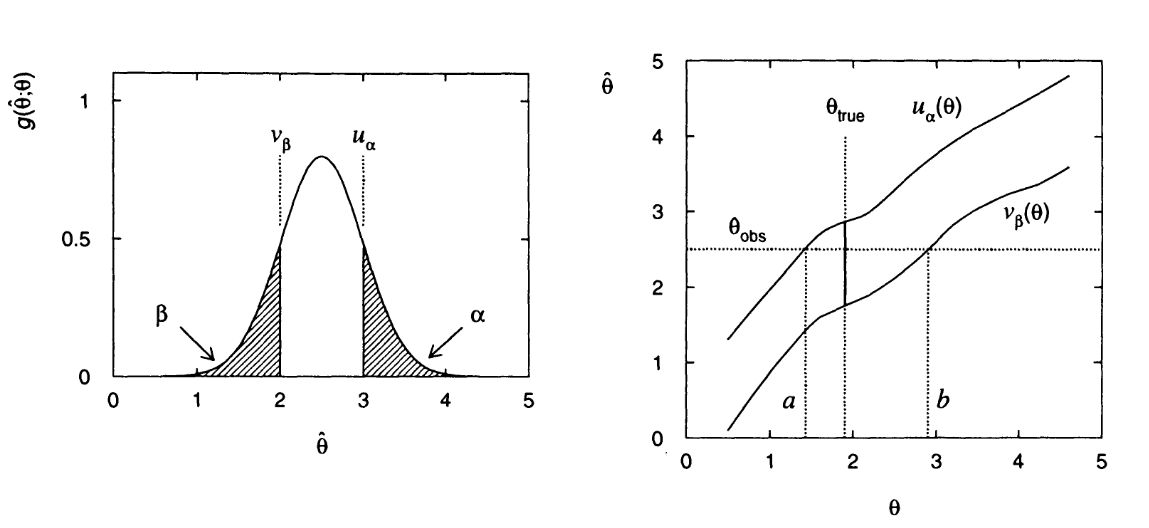
\includegraphics[scale=0.4]{CL_freq}
\caption{Esquema de construcción de un intervalo de confianza frecuentista}
\label{fig:cl_freq}
\end{figure}

El proceso es, dado un estadístico $\hat{\theta}$ con distribución $g(\hat{\theta};\theta)$ (donde queda claro que depende de $\theta$ la distribución). Con esta distribución obtenemos un intervalo con probabilidad $1 - \alpha - \beta$ centrado en la esperanza $E(\hat{\theta})$. Así obtenemos dos pares de puntos, para cada valor de $\theta$. Con eso graficamos un conjunto en el plano $\theta \hat{\theta}$ que denominamos \emph{cinturón de confianza}, que eventualmente contiene el intervalo de confianza, dado el estimador observado. Esto, se resume en la figura \ref{fig:cl_freq}. Si lo queremos escribir, se resume en
\begin{equation}
\begin{gathered}
\alpha = \int_{-\infty}^{u_\alpha} g(\hat{\theta};\theta) d\hat{\theta} \\
\beta = \int_{v_\beta}^{\infty} g(\hat{\theta};\theta) d\hat{\theta}
\end{gathered}
\end{equation}
y determinamos las siguientes funciones, asumiendo que son monotonas crecientes
\begin{equation}
\begin{gathered}
a(\hat{\theta}) = u_\alpha^{-1}(\hat{\theta}) \\
b(\hat{\theta}) = v_\alpha^{-1}(\hat{\theta})
\end{gathered}
\end{equation}
tal que
\begin{equation}
P(a(\hat{\theta}) \leq \theta \leq b(\hat{\theta})) = 1 - \alpha - \beta
\end{equation}
o 
\begin{equation}
\begin{gathered}
p(a(\hat{\theta}) \leq \theta) = \alpha \\
P(b(\hat{\theta}) \geq \theta) = \beta
\end{gathered}
\end{equation}
Para presentar el resultado usamos la siguiente notación
\begin{equation}
\hat{\theta}^{+d}_{-c} = 45^{+2}_{-1}
\end{equation}
tal que $d = \hat{\theta} + b$ y $c = \hat{\theta} - a$.

\subsubsection{Intervalos de confianza de estimadores asintóticamente normales}
Sabemos que los estimadores de máxima verosimilitud son asintóticamente normales, es decir que dado un estimador $\hat{\theta}$ MLE su función de distribución es asintóticamente igual a 
\begin{equation}
g(\hat{\theta};\theta) = \frac{1}{\sqrt{2\pi \sigma_{\hat{\theta}}}} \exp\left[-\frac{(\hat{\theta} - \theta)^2}{2\sigma^2_{\hat{\theta}}}\right]
\end{equation}
La verosimilitud, mientras tanto, es una función $L(\underline{x}|\theta)$, pero la podemos transformar, sin ningún problema, en $L(\hat{\theta}|\theta)$. De esta forma, necesariamente la verosimilitud es asintóticamente
\begin{equation}
L(\hat{\theta}|\theta) = L_{\text{max}} \exp\left[- \frac{(\hat{\theta} - \theta)^2}{2 \sigma^2_{\hat{\theta}}}\right]
\end{equation}
y por lo tanto el logaritmo de la verosimilitud
\begin{equation}
\log L(\hat{\theta}|\theta) = \log L_{\text{max}} - \frac{(\hat{\theta} - \theta)^2}{2 \sigma^2_{\hat{\theta}}}
\end{equation}
que corresponde a una cuadrática. Como $(\hat{\theta} - \theta)^2$ es una variable aleatoria, el logaritmo de la verosimilitud es una variable $\chi^2_{n = 1}$. Esta variable tiene $68\%$ de probabilidad para $x \approx 1$ y $95\%$ para $x \approx 4$, por lo que si elegimos la curvas de nivel
\begin{equation}
\begin{gathered}
\log L = \log L_{\text{max}} - \frac{1}{2} \\
\log L = \log L_{\text{max}} - \frac{2^2}{2}
\end{gathered}
\end{equation}
tiene $68\%$ y $95\%$ respectivamente. Este método también puede usarse para estimadores de cuadrados minimos, que en el caso lineal también son asintóticamente normales, o para cualquier estimador que asintóticamente sea normal. En el gráfico de la figura \ref{fig:Lchi2} corresponde al proceso, donde graficamos menos el logaritmo por una cuestión didáctica.

\begin{figure}[H]
\centering
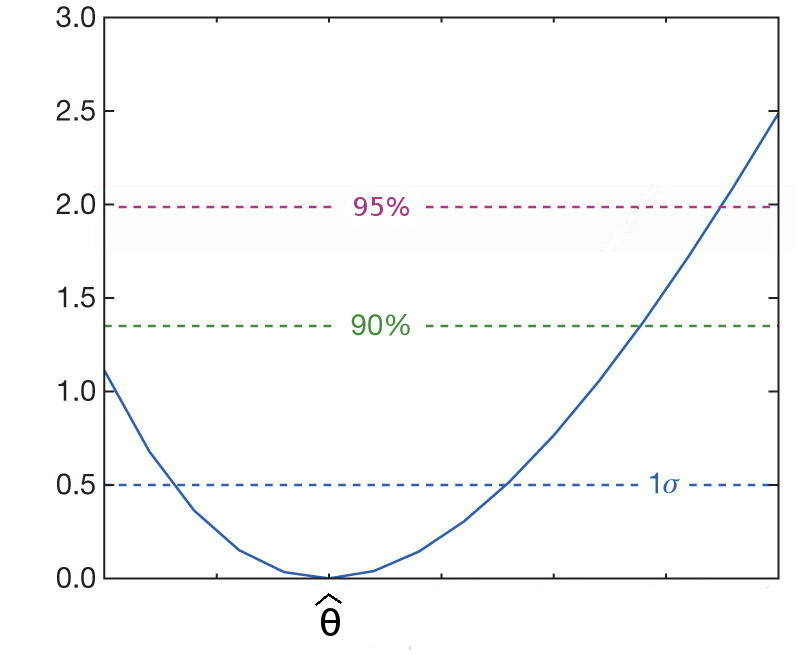
\includegraphics[scale=0.45]{Lchi2}
\caption{Función $\log L(\hat{\theta}(\underline{x})|\theta)$ en función de $\theta$ con el máximo estimador marcado }
\label{fig:Lchi2}
\end{figure}

En caso de tener $n$ variables las curvas de nivel son hiperesferoides de $n-1$ dimensiones, y eventualmente podemos reducirlo siempre a cuadráticas para cada parámetro, por medio de marginalizaciones.

\subsubsection{Intervalos de confianza de los parámetros de datos normalmente distribuidos}
Un caso muy común, cortesía del teorema central del límite, es que los datos $\underline{x}$ provengan de una distribución normal con parámetros $\mu$ y $\sigma$. De esa forma, queremos estimar intervalos de confianza para esos dos parámetros, conocidos o no el otro parámetro.

El caso más simple, que ya comentamos, es la estimación del intervalo de $\mu$ conocido el parámetro $\sigma$. Sabemos que el estadístico 
\[ \overline{X} = \frac{1}{n} \sum_{i = 1}^{N} x_i \]
es el mejor estimador para ese parámetro. Como son sumas de gaussianas, naturalmente tiene una distribución gaussiana $N(\mu, \sigma / \sqrt{n})$ (ver mínima verosimilitud). Con el siguiente cambio de variables
\begin{equation}
\hat{t} = \sqrt{n} \frac{\overline{X} - \mu}{\sigma}
\end{equation}
obtenemos un estimador $\hat{t} \sim N(0,1)$ que corresponde a un pivot, que nos permite determinar el intervalo para $\mu$, haciendo el siguiente despeje
\[ P(\hat{t} < a) = \alpha\]
\[ P\left(\sqrt{n} \frac{\overline{X} - \mu}{\sigma} < a\right) = \alpha \]
\[ P\left(\overline{X} - \mu < a \frac{\sigma}{\sqrt{n}}\right) = \alpha \]
\[ P\left(\mu > \overline{X} - a \frac{\sigma}{\sqrt{n}}\right)  = \alpha \]
donde haciendo una inversión llegamos a una expresión para el extremo inferior, que depende de los datos y la probabilidad del intervalo de confianza. El mismo argumento podemos hacer para el intervalo superior.

Si queremos calcular el intervalo de confianza para $\sigma$ (en este caso $\sigma^2$), conociendo el valor de $\mu$, sabemos que el mejor estimador es
\begin{equation}
S^2 = \frac{1}{N} \sum_{i=1}^{N} (x_i - \mu)^2
\end{equation}
Si multiplicamos por $\frac{N}{\sigma^{2}}$ al estimador tenemos que
\begin{equation}
\frac{N S^2}{\sigma^2} = \sum_{i=1}^{N} \frac{(x_i - \mu)^2}{\sigma^2} \sim \chi^{2}_{(N)}
\end{equation}
donde encontramos nuestro pivot, conociendo $\mu$.

Ahora si no conocemos $\mu$, el estimador más razonable para la varianza es la varianza muestral, es decir
\begin{equation}
s^2 = \frac{1}{N - 1} \sum_{i = 1}^{N} (x_i - \overline{x})^2
\end{equation}
y si lo multiplicamos por $\frac{n - 1}{\sigma^2}$ tenemos que
\begin{equation}
\frac{(N - 1) s^2}{\sigma^2} = \sum_{i = 1}^{N} \frac{(x_i - \overline{x})^2}{\sigma^2} \sim \chi^2_{(N-1)}
\end{equation}
y usamos las mismas herramientas que antes.

Finalmente, si queremos encontrar $\mu$, sin conocer $\sigma$, podemos usar el siguiente pivot
\begin{equation}
\hat{t} = \sqrt{N}\frac{\overline{X} - \mu}{s} \sim t(N - 1)
\end{equation}
donde $s^2$ es la varianza muestral. Este estimador tiene la distribución t de student con $N - 1$ grados de libertad.

\subsection{Intervalos de confianza bayesianos}
En la interpretación bayesiana, la probabilidad consiste en la confianza o seguridad que ese evento. Es fácil demostrar que esa interpretación corresponde una probabilidad, y es fácil también asignarle esa interpretación a la probabilidad axiomática. 
Sin embargo, en la interpretación bayesiana podemos pensar en la distribución del parámetro, que representa la información que conocemos de él. Para eso debemos considerar la verosimilitud como una probabilidad conjunta (aunque sabemos que $L(\theta|\underline{x})$ no está normalizada). Por el teorema de Bayes para variables continuas tenemos que
\begin{equation}
f(\theta|\underline{x}) = \frac{L(\underline{x}|\theta) \pi(\theta)}{\int L(\underline{x}|\theta) \pi(\theta) d\theta}
\end{equation}
donde se denomina \emph{prior} a $\pi(\theta)$, que representa el conocimiento a priori de los parámetros. La verosimilitud representa la información del experimento y la función $f(\theta|\underline{x})$ se denomina \emph{posterior}, que es la función de probabilidad del parámetro. 

El intervalo de confianza $\alpha$CL y la estimación puntual del parámetro, con la distribución posterior, corresponde a un intervalo con probabilidad $\alpha$ y la esperanza de la distribución, respectivamente, es decir
\begin{equation}
\begin{gathered}
E(\theta) = \int \theta f(\theta | \underline{x}) d\theta \\
[a, b] \; / \; P(a \leq \theta \leq b) = \int_a^b f(\theta|\underline{x}) d\theta = \alpha
\end{gathered}
\end{equation}

\section{Test de hipotesis}
Los test de hipotesis corresponden a encontrar un estadístico sensible a la hipótesis, que podemos pensar como un parámetro o no, y definimos una zona crítica para el estadístico, dada una sensibilidad $\alpha$. Esta sensibilidad $\alpha$ corresponde a la probabilidad de rechazar una hipótesis correcta, que es un error de tipo I. El test se dice que rechaza con un nivel de confianza $1 - \alpha$.

Para poder expresar de forma sistemática el resultado de un test de hipótesis definimos el \emph{p-valor} (o \emph{p-value}) como la probabilidad de haber obtenido el valor medido del estadístico o peor, es decir
\begin{equation}
\text{p-valor} = p(\hat{t} \geq \hat{t}_{\text{med}}) 
\end{equation}
Dependiendo del test y el significado del estimador, podemos tener el siguiente caso también
\begin{equation}
\text{p-valor} = p(\hat{t} \leq \hat{t}_{\text{med}})
\end{equation}
que representa la probabilidad de haber obtenido el estadístico medido o menor; o también puede ser ambos casos, donde se elige 
\begin{equation}
\text{p-valor} = 2 \min\{p(\hat{t} \leq \hat{t}_{\text{med}}), p(\hat{t} \geq \hat{t}_{\text{med}})\}
\end{equation}
y que representa los dos casos anteriores, y se denomina a \emph{dos colas}. 

Si el resultado de un test da un p-valor menor a la significancia previamente establecida, podemos rechazar la hipótesis subyacente del estimador elegido. Obviamente, no podemos calcular la probabilidad de una hipótesis dado los datos, ya que no son eventos independientes y es necesario tener información adicional para usar el teorema de Bayes (o sería incurrir a una falacia lógica).  El concepto de p-valor está sumarizado (en un diagrama en inglés lamentablemente) en el diagrama de la figura \ref{fig:p-value}.

\begin{figure}[H]
\centering
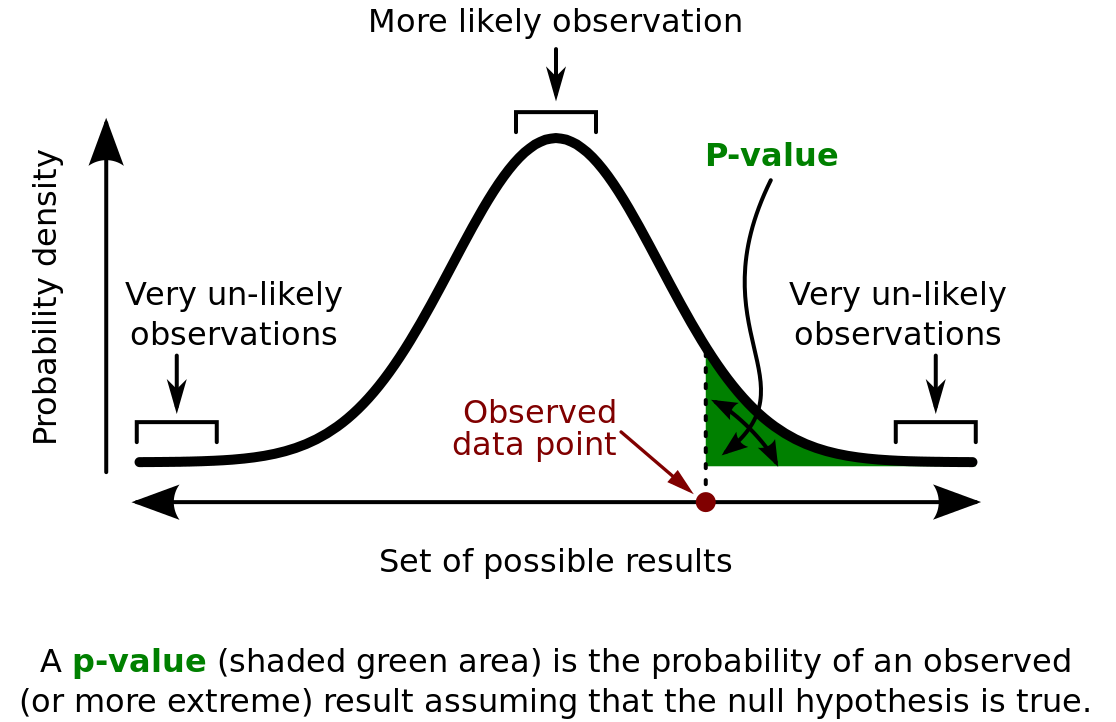
\includegraphics[scale=0.4]{p-value}
\caption{Concepto de p-valor diagramado. Se determina la probabilidad de observar los datos dada la hipotesis}
\label{fig:p-value}
\end{figure}

El p-valor es una variable aleatoria, tal que
\begin{equation}
\text{p-valor} \sim U(0,1)
\end{equation}
Esto es explotado en algunos test, por ejemplo en el Kolmogorov-Smirnov, y también permite juntar dos test independientes para eventualmente tener un test con más poder de resolución.

Vamos a llamar a la hipotesis $H_0$ \emph{hipotesis nula} y otra, que no siempre voy a poder encontrarla, $H_1$, denominada \emph{alternativa}. Estas hipotesis deben ser excluyentes entre si. En la figura \ref{fig:test_h0_h1}, podemos ver un grafico representando la hipotesis y la distribución del estadístico

\begin{figure}[H]
\centering
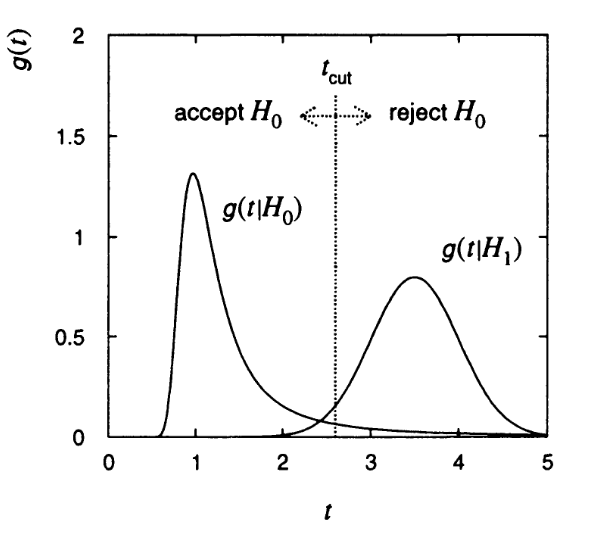
\includegraphics[scale=0.45]{test_h0_h1}
\caption{Distribuciones del estadístico, en un caso paramétrico, con $H_0$ y $H_1$ como válida en cada caso}
\label{fig:test_h0_h1}
\end{figure}

Dada una \emph{región crítica} $C$, es decir $\underline{X} \in C$ implica que se rechaza la hipotesis $H_0$, podemos definir el \emph{poder del test} $\delta$ como
\begin{equation}
\pi(\theta|\delta) = p(\underline{X} \in C | \theta \in \Omega_i)
\end{equation}
siendo $\Omega_i$ la región del parámetro (o el estadístico) que determina la hipotesis $H_i$. Se busca que un test tenga
\begin{equation}
\begin{gathered}
\pi(\theta \in \Omega_0 |\delta) = 0 \\
\pi(\theta \in \Omega_1 | \delta ) = 1
\end{gathered}
\end{equation}
pero vamos a ver que esto es imposible, pero podemos maximizarlo. Se denomina probabilidad de comenter un \emph{error de tipo II} a la probabilidad de $H_0$ de forma incorrecta, ya que la hipotesis $H_1$ es verdadera, es decir esta probabilidad es
\begin{equation}
\beta = 1 - \pi(\theta \in \Omega_1 | \delta)
\end{equation}
En la figura \ref{fig:test_h0_h1} la probabilidad de cometer un error tipo II corresponde al area debajo de la curva de $g(t|H_1)$ de $-\infty$ hasta $t_{\text{cut}}$. 
\subsection{Test paramétrico}
Vamos a ver un caso específico, donde las hipotesis excluyen el parámetro a dos valores posibles. Es decir
\begin{equation}
\begin{gathered}
H_0 : \theta = \theta_0\\
H_1 : \theta = \theta_1
\end{gathered}
\end{equation}

Estos test se llaman \emph{paramétricos} simples. Los test \emph{no paramétricos}, es decir que la hipotesis nula no espera un parámetro si no define una región crítica para un estimador, en general no tienen una hipotesis alternativa, por lo que no podemos usar estos resultados

Ahora, queremos encontrar una zona crítica que maximize el poder en la región $\Omega_1$ y minimize en la región $\Omega_1$, que podemos parametrizar de la siguiente forma
\begin{equation}
\min_{C}\left\{k \pi(\theta_0|\delta) - \pi(\theta_1|\delta)\right\}
\end{equation} 
El valor $k$ está para finalemente setear una significancia y además para pesar el error de tipo I frente al error de tipo II. Como son dos probabilidades, sabemos que dada una verosimilitud
\[ k \pi(\theta_0|\delta) - \pi(\theta_1|\delta) = k \int_{X \in C} L(\underline{x}|\theta_0) d\underline{x} - \int_{X\in C} L(\underline{X}|\theta_1) d\underline{x}\]
como la probabilidad, por lo tanto la verosimilitud es una magnitud positiva, esta última expresión va a ser minima solamente si el integrando es menor a cero, es decir
\[k  L(\underline{x}|\theta_0) - L(\underline{X}|\theta_1) < 0\]
Entonces nos queda definida una región crítica $C$ tal que
\begin{equation}
\frac{L(\underline{x}|\theta_0)}{L(\underline{x}|\theta_1)} > k
\end{equation}
que corresponde a un test LRT (o Likelihood Ratio Test). Esto define una significancia ya que
\begin{equation}
p\left( \frac{L(\underline{x}|\theta_0)}{L(\underline{x}|\theta_1)} > k \right) = \alpha
\end{equation}

Ahora tenemos otro test $\delta^*$, si cumple el minimo de LRT entonces necesariamente es el mismo test. Esto se puede expresar como
\[ k \pi(\theta_0|\delta) - \pi(\theta_1|\delta) < k \pi(\theta_0|\delta^*) - \pi(\theta_1|\delta^*)\]
si reordenamos los términos encontramos que
\[ \pi(\theta_1|\delta) > \pi(\theta_1|\delta^{*}) + k( \pi(\theta_0|\delta) - \pi(\theta_1|\delta^{*})) \]
lo que nos determina que si
\begin{equation}
\pi(\theta_0|\delta) \leq \pi(\theta_1|\delta^{*}) \; \Rightarrow \; \pi(\theta_1|\delta) \geq \pi(\theta_1|\delta^{*})
\end{equation}
Es decir, dado un test con menor o igual significancia, entonces el poder está acotado por el test LRT. El límite de la significancia es importante, ya que uno puede exigir significancia $\alpha = 1$, pero implicaría necesariamente poder nulo (que es absurdo para un test).

Estos resultados pueden ser extendidos a test \emph{compuestos}, donde las hipótesis separan regiones del espacio de parámetros, usando el supremo de la verosimilitud

\end{document}


